% !Mode:: "TeX:UTF-8"
% !TEX program  = xelatex


\documentclass{cumcmthesis}
\usepackage[framemethod=TikZ]{mdframed}
\usepackage{url}   % 网页链接
\usepackage{subcaption} % 子标题
\usepackage{float}
\usepackage{enumitem}

\begin{document}

\tableofcontents

\newpage
\section{问题重述}
\subsection{问题背景}
农村供水范围和管道铺设规模正随着我国城镇化的不断的发展而逐渐扩大,并且农村居民对日用水定额以及水质的要求随着生活质量的提升而逐渐增加,因此如何保证供水质量及方便设备维护成为研究问题之一。为使管道铺设总里程最短,最小生成树(Minimum Spanning Tree,MST)算法首选。经典的最小生成树问题可描述为:在一给定的无向图G=(V,E)中,(u,v)代表连接顶点u与顶点v的边,而w(u,v)代表此边的权重,若存在T为E的子集且为无循环图,使得w(T)最小,则此T为G的最小生成树。由于其在交通运输、城市规划、经济管理等领域应用广泛,衍生出了众多研究分支,度约束最小生成树(Degree-Constrained Minimum Spanning Tree,DCMST)问题就是其中一种重要的扩展类型。解决该问题的常用算法有Kruskal算法和Prim算法,通过对比两种算法的时间复杂度、空间复杂度、贪心策略以及算法实现过程中图的状态,从算法选择的角度得出结论:在图结构中边数较少时采用Kruskal算法,边数较多时采用Prim算法较合理。

由于本题最小生成树边数较多,根据Kruskal算法的执行过程得知,边数较多时,为了减少时间复杂度,不易采用Kruskal最小生成树算法。相反Prim算法在执行过程中无需对边线排序,只与树中的顶点有关,因为它是每次加一个顶点,对边数多时使用,因此本题采用Prim算法。


\subsection{问题提出}
中心供水站(类型A)、12个一级供水站(类型V)和168个二级供水站(类型P)的地理坐标已确定。中心供水站只能和一级供水站连接,一级供水站之间可连接,均铺设I型管道;一级供水站可以和二级供水站连接,二级供水站之间可连接,均铺设II型管道。各级供水站之间的连接管道必须从上一级供水站或同一级供水站的位置坐标出发,且两供水站之间长度可简化为欧氏距离,这表明两供水站之间的距离定义为

针对上述管道铺设要求,解决以下问题:
\begin{itemize}
    \item 问题1:从中心供水站出发,用图呈现使I型管道和II型管道总里程数最小的方案,并计算I型管道和II型管道总里程数。
    \item 问题2:升级两个二级供水站为一级供水站,使II型管道总里程数最小;与问题1进行比较,计算II型管道减少的里程数。
    \item 问题3:在问题1基础上,由于功率影响,从一级供水站出发铺设的管道最多只能供水40公里,但从中心供水站A出发铺设的管道供水不受此距离限制。请设计方案至少升级几个二级供水站为一级供水站,可实现对所有的供水站供水,并计算在此配置下最小总里程数。
\end{itemize}

\section{问题分析}

\subsection{问题一的分析}
问题一首先要求我们根据各一级供水站和二级供水站的位置信息,寻找到使铺设各级管道总里程最少的方案。由于铺设条件的约束:中心供水站只能连接一级供水站,一级供水站可以连接一级和二级供水站,二级供水站只能连接二级供水站,且管道必须在各级供水站内部铺设,即不能在管道之间连接新的管道。因此,首先需要解决中心供水站到一级供水站的管道铺设问题,然后根据已经铺设好的一级管道分布,选择二级管道的铺设方式。这是一个经典的最小生成树问题,各级供水站之间的距离即为边的权重。

首先,我们利用个供水站的分布数据求得可能出现的管道铺设方式的里程数,通过Prim算法依次连接各一级供水站,Prim算法会找出加权值最小的候选边线并将其添加到树结构中,这样就可以求得一级管道的最短铺设里程。然后将整个供水系统看做一个生成树,重复上述工作,可求出整体管道铺设总里程数以及二级管道的铺设总里程数。

\subsection{问题二的分析}
问题二要我们考虑在二级管道供应不足的情况下,如何通过提升供水站的等级使得铺设的二级管道总里程减少。在共168个二级供水站中选择两个升级为一级供水站,这样供水站布局变为14个一级供水站和166个二级供水站。

首先,我们通过分析166个二级供水站的地理坐标,研究升级某个二级供水站对管道体系的影响。我们还要同时考虑到升级供水站后的实际效果,如果升级后的一级供水站不能为任何二级供水站供水或者会导致铺设管道里程总数的上升,升级后的效果可能不够理想。我们希望找到一种既能减少二级管道铺设里程数并且还能满足实际使用的方案。

\subsection{问题三的分析}
问题三考虑到功率的影响,从一级供水站出发铺设的二级管道总里程长度最多只能供水40公里,这时要考虑到对二级供水站的升级,我们首先分析在没有升级的情况下,从各一级供水站出发铺设的二级管道总里程的情况。


\begin{figure}[!h]
  \centering
  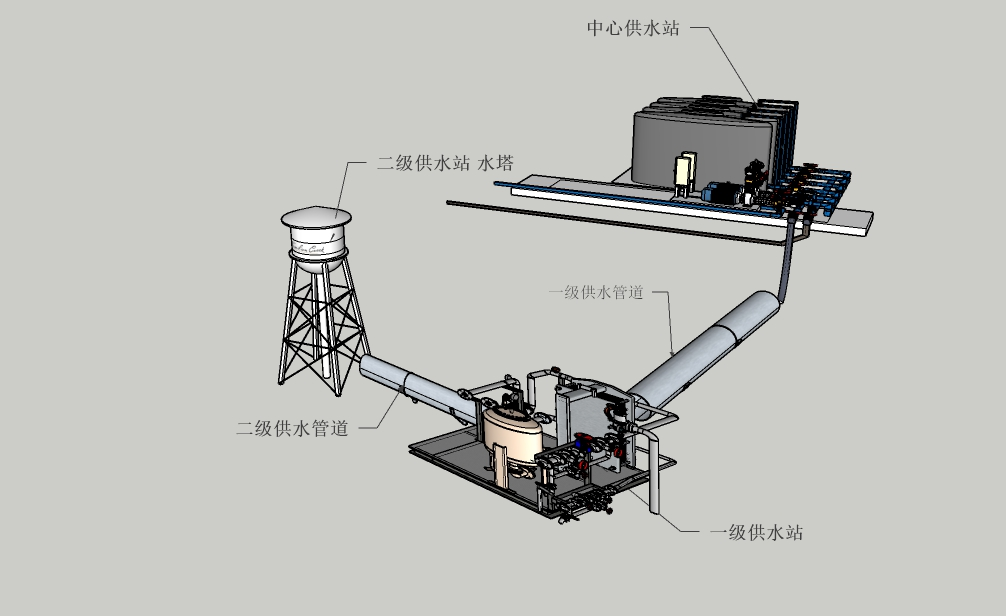
\includegraphics[width=.6\textwidth]{figure/shuiguan.jpg}
  \caption{供水系统的3d示意图}
    \label{fig:circuit-diagram}
\end{figure}



\section{符号说明}
\begin{center}
  \begin{tabular}{cc}
      \toprule[1.5pt]
      \makebox[0.3\textwidth][c]{符号}	&  \makebox[0.4\textwidth][c]{意义} \\ \midrule
      $A$	    &中心供水站\\ 
      $N_1$         &一级供水站的数量\\	
      $N_2$         &二级供水站的数量\\	
      $V[i]$	    &一级供水站$i=1,2,...N_1$\\ 
      $P[i]$	    &二级供水站$i=1,2,...N_2$\\ 
      $distanceMat[i,j]$	    &第i,j个供水站之间的距离,$i,j=1,2,...,N_1+N2+1$\\ 
      $V,E$	    &各级供水站的集合或各供水站可能的连接情况的集合\\ 	
      $w$	    &各连接管道的权重\\ 
      $TL_{i}$    &从各一级供水站出发的二级管道总长度,$i=1,2,...N_1$\\ 
      $h$         &需要嫁接树苗的总数\\
      $q_{i}$     &相应树苗上的节点总数\\
      $b_{iq_{i}}$	    &各分支管道系统上的二级供水站的编号,$i=1,2,...N$\\ 
     
      \bottomrule[1.5pt]
  \end{tabular}
\end{center}

\section{模型假设}
\begin{itemize}
  \item 假设所有供水站处于同一水平面,即不考虑各级供水站之间的地形、地貌等因素影响,即供水站之间铺设的管道长度为其之间的欧氏距离。
  $$\sqrt{(\Delta x)^2+(\Delta y)^2}$$
  \item 各级水管之间允许在空间上交叉,且地下布置管线的深度差别对长度的影响忽略不计。
  \item 水源从中心供水站流向一级供水站,再流向二级供水站。每个供水站只有一个输入管道,可以没有或者有多个输出管道。
\end{itemize}

\section{问题1的模型建立与求解}
\subsection{问题1的描述与分析}
  问题一首先要求我们根据表格中给定的各级供水站的坐标,确定管道的铺设计划以使各级管道的铺设里程数最小,首先,为了清晰直观地观察每个供水站的位置,我们用matlab绘制了各级供水站的坐标示意图,将不同级别的供水站分别标注出来。
  管道的铺设遵循以下技术规定:
\begin{itemize}
    \item 各级供水站逐级连接,中心供水站只能与一级供水站连接,一级供水站可以和二级供水站连接。
    \item 同级供水站可以相互连接,即一级供水站可以与一级供水站连接,二级供水站可以与二级供水站连接。
    \item 各级供水站之间的接连管必须从上一级供水站或同一级供水站的坐标位置出发,即不能在管道中间随意连接其他管道。
\end{itemize}

在本题中,中心供水站位于12个一级供水站坐标的几何中心区域,我们画出了各一级供水站到中心供水站及一级供水站之间距离的联通图:
\begin{figure}[!h]
  \centering
  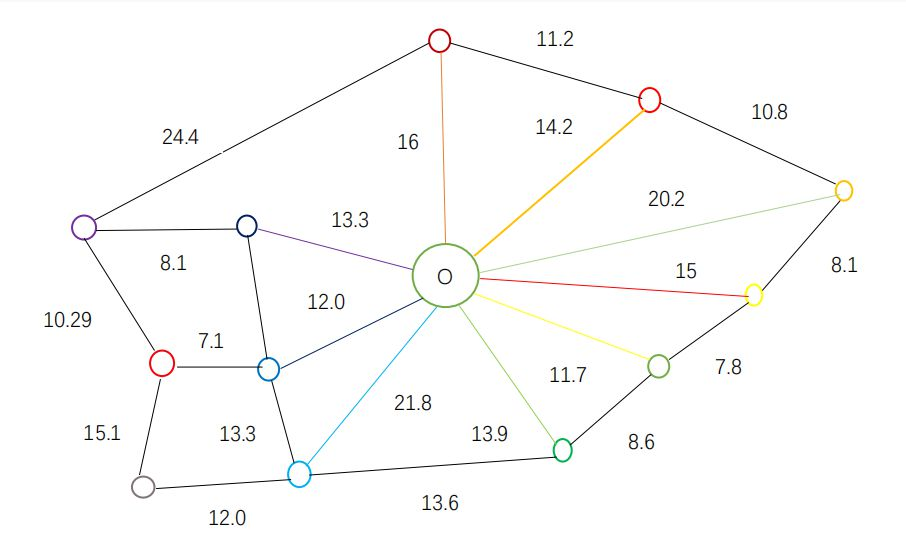
\includegraphics[width=.6\textwidth]{figure/a.jpg}
  \caption{连通图}
  \label{fig:circuit-diagram}
\end{figure}

\subsection{问题1模型的建立}
我们可以将上述管道铺设问题用一个连通无向图$G=(V,E)$来表示,这里的$V$是针脚的集合,$E$是针脚之间的可能连接,并且对于每条边$(u,v)\in E$,我们为其赋予权重$w(u,v)$作为连接针脚$u$和针脚$v$的代价,我们希望找到一个无环子集$T\subset E$,既能够将所有节点连接起来,又具有最小的权重,即
$$w(T)=\sum\limits_{(u,v)\in T}{w(u,v)}$$
的值最小。由于$T$是无环的,而且连通所有的节点,因此,$T$必然是一个树形物。我们称这样的树为生成树,为求管道铺设的最短里程,即要求铺设管道的最小生成树。在本题中,我们用两供水站之间的距离表示线的权重:
$$L(u,v)=\sqrt{(x_{u}-x_{v})^{2}+(y_{u}-y_{v})^{2}}$$

贪心策略:
集合$A$是某最小生成树的一个子集,总是保持无环状态。若将边$(u,v)$加入到集合$A$中,使得$A$不违反循环不变式,即$A\cup{(u,v)}$也是某棵最小生成树的子集,则称该边为安全边。该策略应符合一下规则:
\begin{itemize}
  \item 算法执行的任何时刻,图$G_{A}=(V,A)$是一个森林,$G_{A}$中的每个连通分量是一棵树,算法开始时,集合$A$为空集,森林中包含$|V|$棵树,每棵树只有一个节点。
  \item 对于集合$A$为安全的边所连接的是$G_{A}$中不同的连通分量,因此每执行一次循环,减少一棵树。
  \item 循环共执行$|V|-1$次,当整个森林仅包含一棵树时,终止循环。
\end{itemize}

\subsubsection{Prim算法}
  Prim算法是从单个起始点构成的树结构开始,向树结构逐条添加边线以生成树。也就是说,Prim最小生成树是从一个具有n个顶点的带权无向完全图中选择n-1条边并使这个图连通,同时使生成树的权值最小。Prim算法从图中的一个顶点开始,把这个顶点包含在一个集合中,反复寻找一个顶点已在该集合中而另一个顶点还不在该集合中的最小权边,把新边和新节点归并到生成树中,找到这个连通图的最小生成树。在连接节点边数较多时,使用Prim算法较为合适。

  集合A是一棵树,每次加入到A中的安全边永远是连接A和A之外某个节点的边中权重最小的边,采用广度优先搜索的思想——当从Q中取出一个点u时,即要检查u的所有相邻的点,并更新相关的点,Prim算法与分支限界法类似,利用广度优先搜索和优先队列思想,只不过是没有使用分支限界思想。因为可以证明贪心选择性质,使之可以组成一个最优解。
  
\begin{itemize}
  \item 输入:一个加权连通图,其中顶点集合为$V$,边集合为$E$;

  \item 初始化:$Selected = \{x\}$,其中x为集合V中的任一节点(起始点),$Edges = \{\}$,为空;
  
  \item 重复下列操作,直到$Selected = V$:
  \begin{itemize}
    \item 选取权值最小的边$<u, v>$,其中$u \in Selected$,而$v \in V-Selected$;
  
    \item 将$v$加入集合$Selected$中,将$<u, v>$边加入集合$Edges$中;
  \end{itemize}
  \item 输出:使用边集$Edges$来描述所得到的最小生成树。
\end{itemize}

\subsubsection{分级Prim算法}
由于一级水站只能又中心供水站或者其他一级供水站供水,所以我们采用分两级的Prim算法:
\begin{itemize}
  \item 1级Prim算法:输入$V = \{A\}\bigcup \{ V[i]|i=1,2,...N_1\}$,初始化$Selected = \{A\}$。
  输出:边集$Edges1$

  \item 2级Prim算法:输入$V = \{V[i]|i=1,2,...N_1\} \bigcup \{A[i]|i=1,2,...N_2\}$,初始化$Selected = {A}$。输出:边集$Edges2$
  \item 使用边集$Edges1, Edges2$来描述所得到的整个最小生成树。
\end{itemize}
\subsection{问题1模型的求解}
  根据题目要求,我们求出了使得各级管道铺设距离最小的建设方案,如\cref{fig:solution1}所示:
  \begin{figure}[!h]
    \centering
    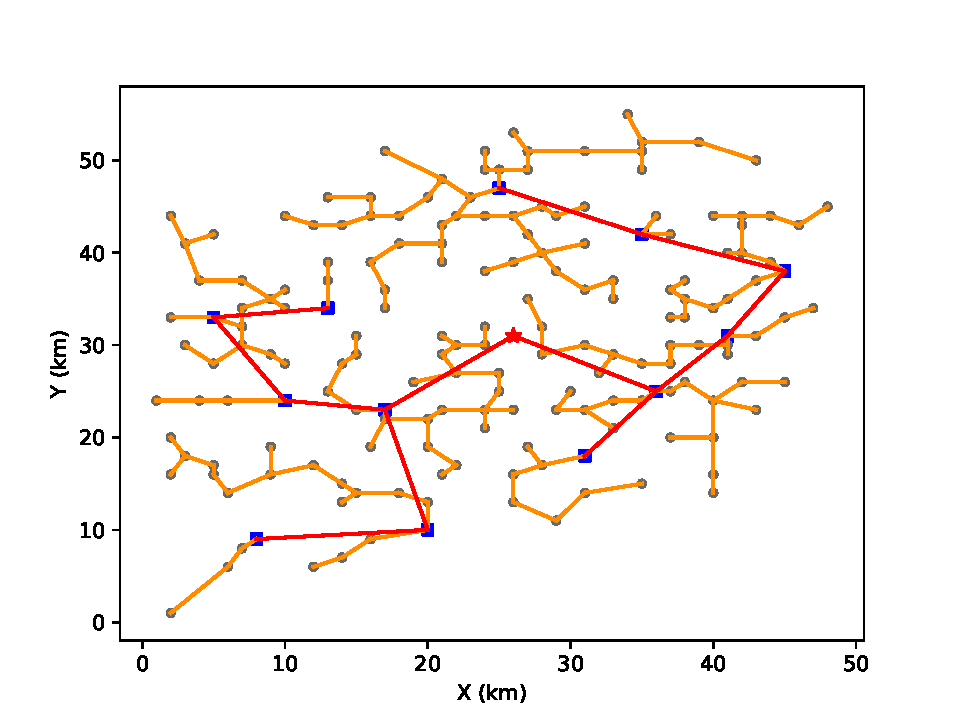
\includegraphics[width=.9\textwidth]{figure/pipeline.pdf}
    \caption{问题1结果}
    \label{fig:solution1}
  \end{figure}

我们还求得从各一级供水站输出的二级供水站个数以及的输出线路的总长度,如\cref{tab:001}所示;

\begin{table}[!h]
  \caption{每个一级供水站供给的二级供水站数量及其所属管道长度}\label{tab:001} \centering
  \begin{tabular}{ccccccccccccc}
      \toprule[1.5pt]
      水站id & 1 & 2 & 3 & 4 & 5 & 6 & 7 & 8 & 9 & 10 & 11 & 12\\
      \midrule[1pt]
      子站个数&16 & 3 & 3 & 2 & 24 & 17 & 46 & 7 & 2 & 16 & 15 & 17 \\
      线路总长&38.95 & 10.05 & 9.0 & 5.0 & 53.68 & 42.8 & 112.40 & 21.97 & 4.23 & 39.94 & 33.09 &32.25  \\
      \bottomrule[1.5pt]
  \end{tabular}
\end{table}

  经过加总可知:最优方案建设需要的最少一级管道总里程为120.94km,最少二级管道总里程为403.40km.


\section{问题2的模型建立与求解}
\subsection{问题2的描述与分析}
问题二要求我们在考虑二级管道供应不足的情况下,将两个二级供水站升级为一级供水站,使II型管道总里程数最小,此时供水站布局变为14个一级供水站和166个二级供水站。首先,我们遍历所有二级供水站,选择任意两个供水站进行升级,求得升级后二级管道铺设的总里程数,并计算II型管道减少的总里程数。除此之外,应考虑升级某两个供水站后的实际效果。我们希望找到既减少II型管道总里程数,又实用的方案。

\subsection{问题2模型的建立}
  在某一连通无向量图$G=(V,E)$中共有N个不同类型的站点,无环子集$T\subset E$,既能够将所有节点连接起来,又具有最小的权重,即$w(T)=\sum\limits_{(u,v)\in T}{w(u,v)}$的值最小。由于$T$是无环的,而且连通所有的节点。此时,连接各站点的边的总数共有$sum=N-1$条。
  所以我们给出推论\cref{corollary:001}
  \begin{corollary}
    若对$m$个二级供水点进行升级,相应的一级管道数量会增加$m$个,二级管道会减少$m$个。
    \label{cor:001}
  \end{corollary}

  本题中含有共181个供水站,其中中心供水站一个,一级供水站12个,二级供水站168个,按照生成树的生成规则,连通各级站点,得一级管道12条,二级管道168条。

  我们发现在对二级供水站进行升级后,包含该站点的最新最小生成树,将在新站点和与其相距最近的一级站点或中心站点之间建立新的一级管道,并自动取消其与最近的二级站点之间的二级管道建设。
  \cref{fig:sample-figure-a}和\cref{fig:sample-figure-b}展示了站点的升级如何影响管道铺设情况:
  其中三角形站点代表中心供水站,红色圆形站点代表一级供水站,蓝色圆形站点代表二级供水站:

  \begin{figure}[!h]
    \centering
    \begin{minipage}[c]{0.4\textwidth}
        \centering
        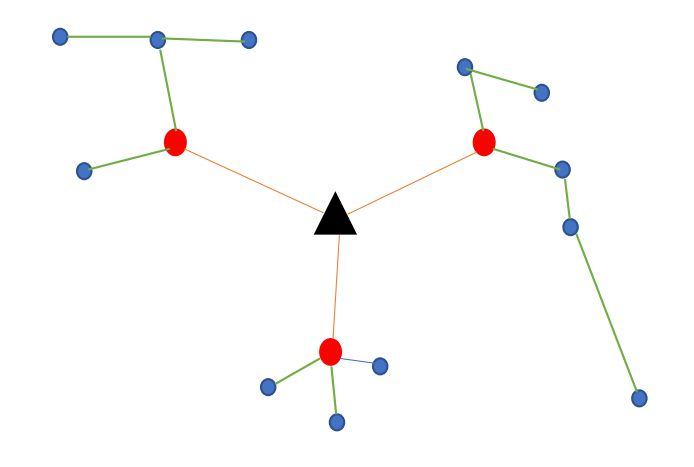
\includegraphics[width=0.95\textwidth]{figure/b.jpg}
        \subcaption{升级前}
        \label{fig:sample-figure-a}
    \end{minipage}
    \begin{minipage}[c]{0.4\textwidth}
        \centering
        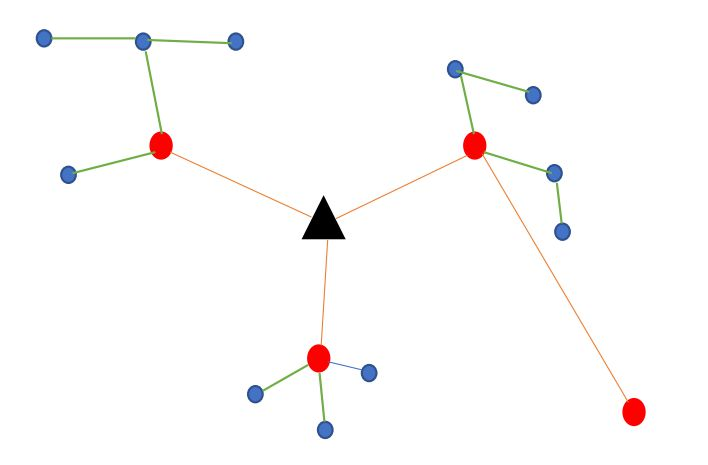
\includegraphics[width=0.95\textwidth]{figure/c.jpg}
        \subcaption{升级后}
        \label{fig:sample-figure-b}
    \end{minipage}
    \label{fig:sample-figure}
  \end{figure}
可见我们升级任何一个二级供水站时$P$,减少的一条II型管道为原先输入$P$的II型管道。
所以此题的解决步骤为:
\begin{itemize}
  \item 将边集$Edges2$中所有管道长度求出,降序排列
  \item 取出$Edges2$中所有管道长度最长的两根管道$E_1,E_2$,升级这两根管道端点中的子节点。
  \item 在$Edges2$中删除II型管道$E_1,E_2$。
  \item 使用Prim算法重新对一级送水站进行布线。
\end{itemize}

\subsection{问题2模型的求解}
问题2模型的解决方案如\cref{fig:solution2}所示。分别升级89, 125号二级供水站,在图中用绿色“+”号标出。
  \begin{figure}[!h]
    \centering
    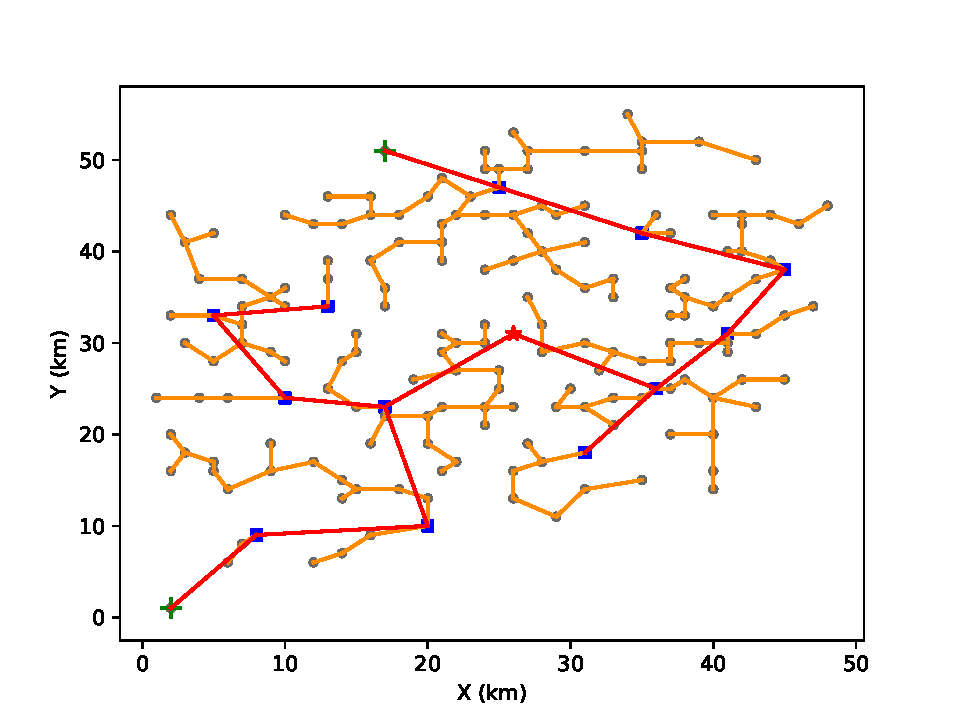
\includegraphics[width=.9\textwidth]{figure/pipelineAfterUpgrade.pdf}
    \caption{问题1结果}
    \label{fig:solution2}
  \end{figure}
  升级两个二级水站后的II型管道总长度为392.00km。相比问题1的长度减少了11.40km。


\section{问题三的模型建立与求解}
\subsection{问题三的描述与分析}
  在不升级任何二级供水站时,所有一级供水站面临的连接和负载情况,已在问题1中得出,如\cref{tab:001}所示:

    从中我们可以发现在该供水系统中,二级供水站与一级供水站的分布位置极不匹配,在第7号一级供水站周围的二级供水站过多,已经给一级供水站增加了许多负担,5、6号一级供水站铺设出的二级管道也超出了范围限制。
    我们接下来会对5、6、7号一级供水站周围的二级供水站进行细分或重新分配,希望保持升级数量较少的同时,满足功率限制。

\subsection{管道分支嫁接模型的建立}
  \subsubsection{最优子结构定理}
    \begin{theorem}
      最优子结构定理:如果一个问题的最优解中包含了子问题的最优解,则该问题具有最优子结构。
      \label{thm:best_sub}
    \end{theorem}
    
    证明如下:假设我们已经得到了一个最小生成树$T$,$(u,v)$是这棵树中的任意一条边,如\cref{fig:mst}所示:
    
    \begin{figure}[!h]
      \centering
      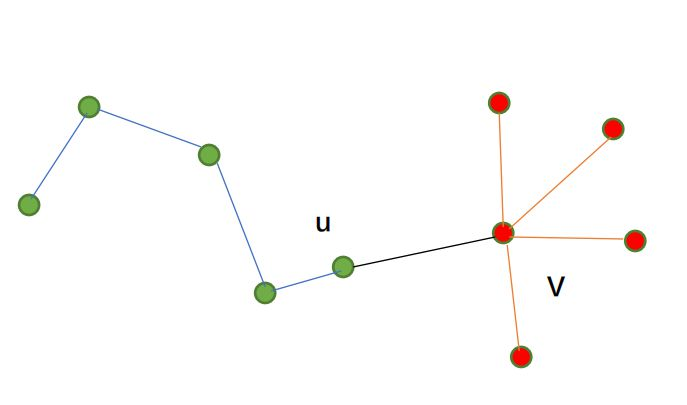
\includegraphics[width=.8\textwidth]{figure/mst.jpg}
      \caption{最小生成树}
      \label{fig:mst}
    \end{figure}
    
    当把连接$u$,$v$的边去掉后(这条边是连接两棵树的最小边),得到两颗子树,如\cref{fig:mst_split}和。
    
    \begin{figure}[!h]
      \centering
      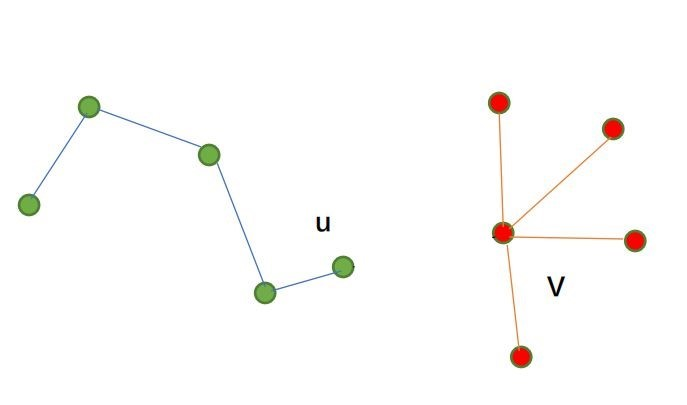
\includegraphics[width=.8\textwidth]{figure/mst_split.jpg}
      \caption{最小生成树的两颗子树}
      \label{fig:mst_split}
    \end{figure}
    
    $T_{1}$是图$G_{1}=(V_{1},E_{1})$的最小生成树,$G_{1}$是由$T_{1}$的顶点导出的图$G$的子图,$E_{1}={(x,y)\in E,x,y\in V_{1}}$同理可得$T_{2}$是$G_{2}=(V_{2},E_{2})$的最小生成树,$G_{2}$是由$T_{2}$的顶点导出的$G$的子图,
    $E_{2}={(x,y)\in E,x,y\in V_{1}}$
    结论证明:使用剪贴法,$w(T)$表示$T$树的权值和。
    权值关系满足:$$w(T)=w(u,v)+w(T_{1})+w(T_{2})$$
    假设有一棵树$T_{1}'$比$T_{1}$更适合图$G_{1}$,那么就存在$T'={(U,V)}\bigcup T_{1}'\bigcup T_{2}'$,那么$T'$就比$T$更适合图$G$,这与$T$是最优解相矛盾,\cref{thm:best_sub}得证。
    

    为了尽可能减少供水站的升级数,我们首先想到的是将超载供水站的连接负载重新分配,每个一级供水站的管道铺设情况已经如上图所示。

    在共$N$个一级供水站中,按照方案一中的管道建造计划,我们将每个管道子系统看做一棵树苗,对其枝条总长度,即二级管道总里程$TL_{i}(i=1,2...N)$进行由小到大的排序,若$TL_{i}>TL_{P},TL_{P}=40km$,则该树苗为被嫁接树苗,即需要减少管道总里程,其余树苗为嫁接树苗,需要平衡负载即增加管道长度。
    对嫁接树苗进行由小到大的重新排序,编号为$a_{1}$,$a_{2}$,....$a_{h}$,$h$为需要嫁接的树苗总数,其相应节点(二级供水站)编号$b_{i1}$,$b_{i2}$,....$b_{iq_{i}}$, $q_{i}$为相应树苗上的节点总数。
    根据两点间距离公式和最优子结构定理,我们在某一嫁接树苗上找到其与被嫁接树苗距离最近的节点,即使某一嫁接树苗上的节点与被嫁接树苗上的节点距离最近的一条线,根据最优子结构定理,嫁接部分可以沿着原线路继续延伸或者寻找新的被嫁接树苗上的节点。
  
    \begin{itemize}
    \item 新树苗需满足功率限制:
    $$TL_{i}'<=TL_{P}$$
    $TL_{i}'$为新树苗的枝条总长度,即新管道分支系统的总里程。
    \item 最佳的新树苗需满足枝条长度达到最长,即不会有其他任何可行的其他连接方式,使得该树苗的长度进一步增加而满足功率限制。
    
    \end{itemize}

    如果所有嫁接树苗都已达到最佳长度,仍有至少一个树苗不满足功率限制,则此时,应对系统进行升级。
 
\subsection{问题三模型的求解}
  各水站负载线路总长度,即所有一级供水站和二级管道输出II级水管线路总长度示意图如\cref{fig:pipline_length}。
  \begin{figure}[!h]
    \centering
    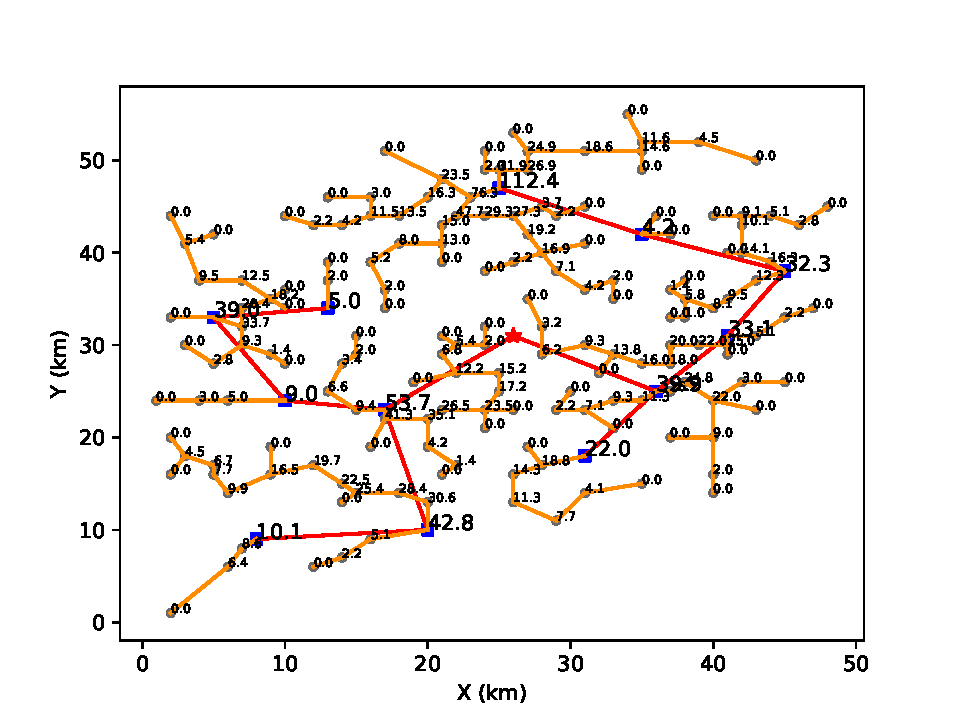
\includegraphics[width=.8\textwidth]{figure/pipline_length.pdf}
    \caption{各水站负载线路总长度}
    \label{fig:pipline_length}
  \end{figure}
  嫁接开始前先求出所有超载的一级水站和其所有子水站列表$overloadStation[]$,此列表长度为超载的一级水站的个数,每个元素为一个集合,包含一级水站和其所有子水站。

  开始第一步嫁接,先求出所有负载未达最大负载$MAX_LOAD$的一级水站和其所有子水站$availableStation[]$,此列表长度为有余闲的一级水站的个数,每个元素为一个集合,包含一级水站和其所有子水站。按照其余闲的负载$availableLoad[]$降序排列。
  
  从余闲的负载最大的一级水站$availableIStation[i]$开始遍历$availableIStation[]$在\cref{fig:pipline_graft_connection_0}。$availableIStation[i]$如图\cref{fig:pipline_graft_connection_0}中绿色圈所示。
  
  下面筛选可能与$availableIStation[i]$嫁接的所有超载树中的水站。
  筛选出二级水站的集合为:
  $$overloadStation={P[i] |P[i].load < availableIStation[i].availableLoad }$$
  即$P[i]$的负载小于可嫁接树的剩余负载。如图\cref{fig:pipline_graft_connection_0}中红色圈所示。

  选取权值最小的边$<u, v>$,其中$u \in availableIStation[i]$,而$v \in overloadStation$
  作为嫁接的连接点。如图\cref{fig:pipline_graft_connection_0}中绿色虚线所示。

  \begin{figure}[!h]
    \centering
    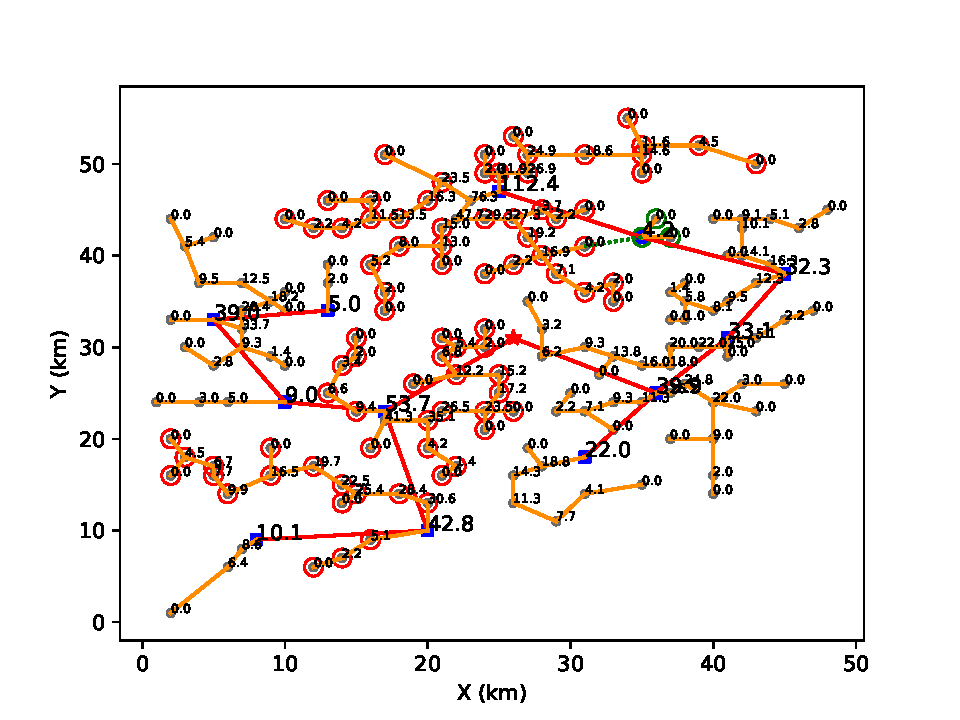
\includegraphics[width=.95\textwidth]{figure/pipline_graft_connection_0.pdf}
    \caption{第1次嫁接的候选水站和执行嫁接连接的两个水站}
    \label{fig:pipline_graft_connection_0}
  \end{figure}
  从$v$开始逐渐追溯其父节点(输入水源的供水站),搜索嫁接部分和超载树之间的切割边$cutEdge=<u_c, v_c>$。使$cutEdge$满足:
  $$u_c.load + distanceMat[u, v]>availableIStation[i].availableLoad$$
  $$v_c.load + distanceMat[u, v]<=availableIStation[i].availableLoad$$
  $cutEdge$中,$u_c$为父节点,$v_c$为子节点,即水流从$u_c$流向$v_c$。$cutEdge$如图\cref{fig:pipline_graft_cut_0}中用无橙色底色的绿色虚线所示。
  \begin{figure}[!h]
    \centering
    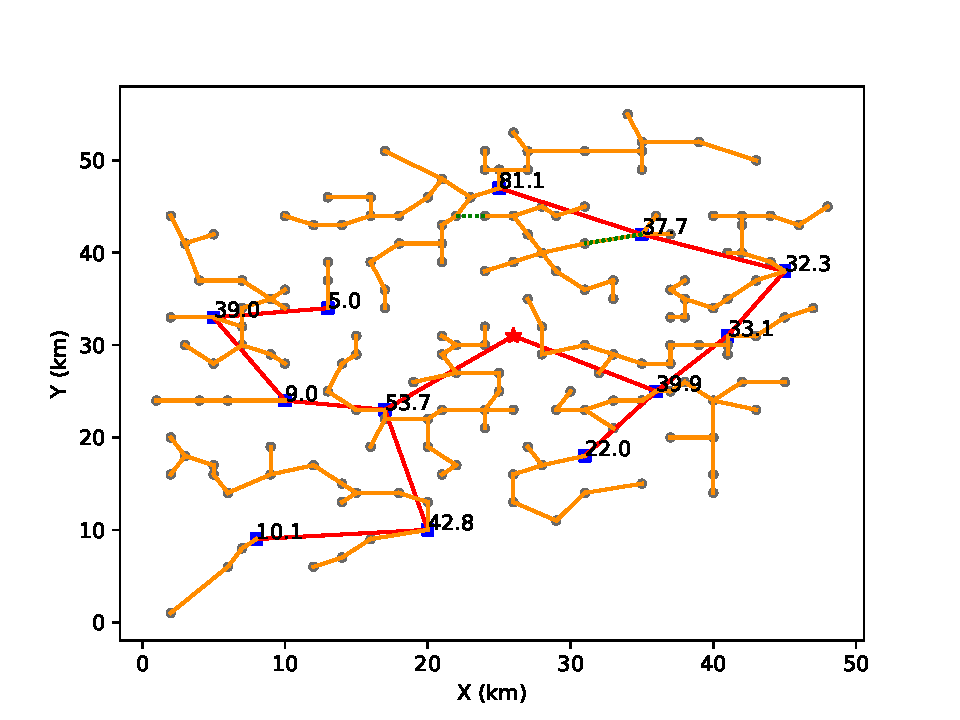
\includegraphics[width=.95\textwidth]{figure/pipline_graft_cut_0.pdf}
    \caption{第1次嫁接断开的边以及嫁接后个一级水站的负载}
    \label{fig:pipline_graft_cut_0}
  \end{figure}

  到此为止视为完成一次嫁接,更新一次所有水站的连接状态树后:
  \begin{itemize}
    \item 更新最小生成树树的连接结构参数。
    \item 更新$overloadStation[]$和$availableIStation[i]$
  \end{itemize}
  遍历进行第二次嫁接,结果如\cref{fig:pipline_graft_connection_1},\cref{fig:pipline_graft_cut_1}。

  \begin{figure}[!h]
    \centering
    \begin{minipage}[c]{0.45\textwidth}
        \centering
        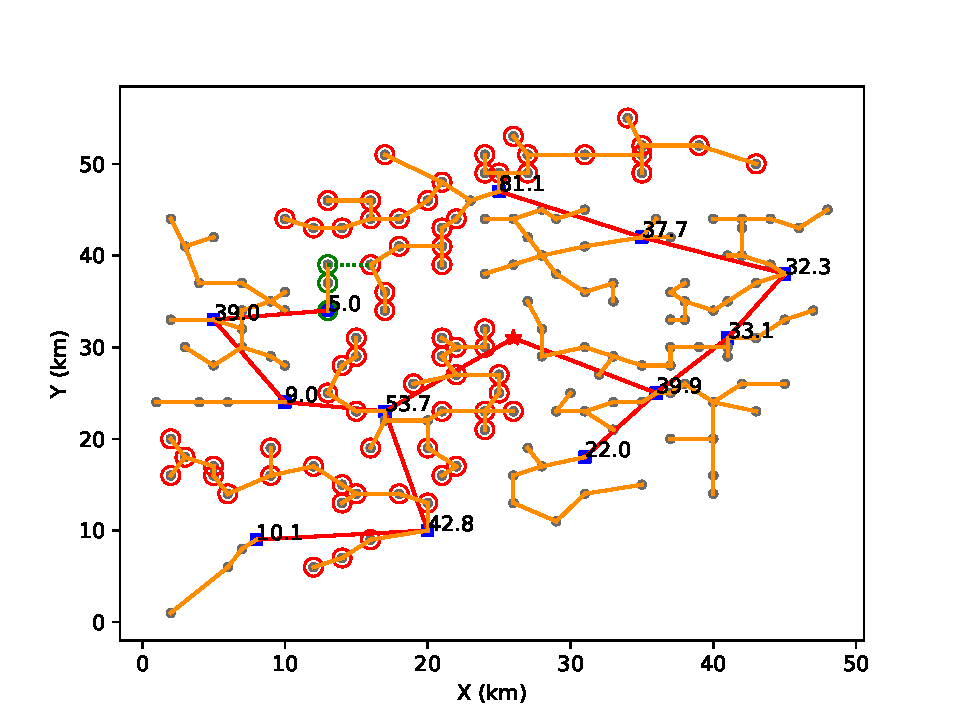
\includegraphics[width=0.99\textwidth]{figure/pipline_graft_connection_1.pdf}
        \subcaption{第2次嫁接的候选水站和$<u, v>$}
        \label{fig:pipline_graft_connection_1}
    \end{minipage}
    \begin{minipage}[c]{0.45\textwidth}
        \centering
        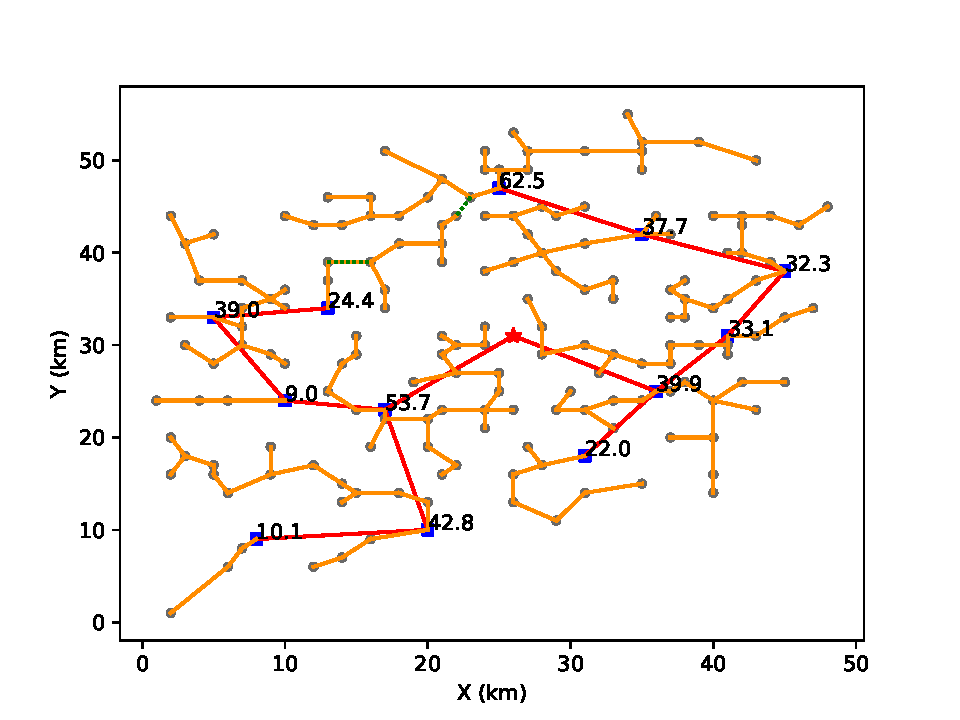
\includegraphics[width=0.99\textwidth]{figure/pipline_graft_cut_1.pdf}
        \subcaption{第2次嫁接断开的边}
        \label{fig:pipline_graft_cut_1}
    \end{minipage}
  \end{figure}
  第3到8次嫁接。

  \begin{figure}[!h]
    \centering
    \begin{minipage}[c]{0.45\textwidth}
        \centering
        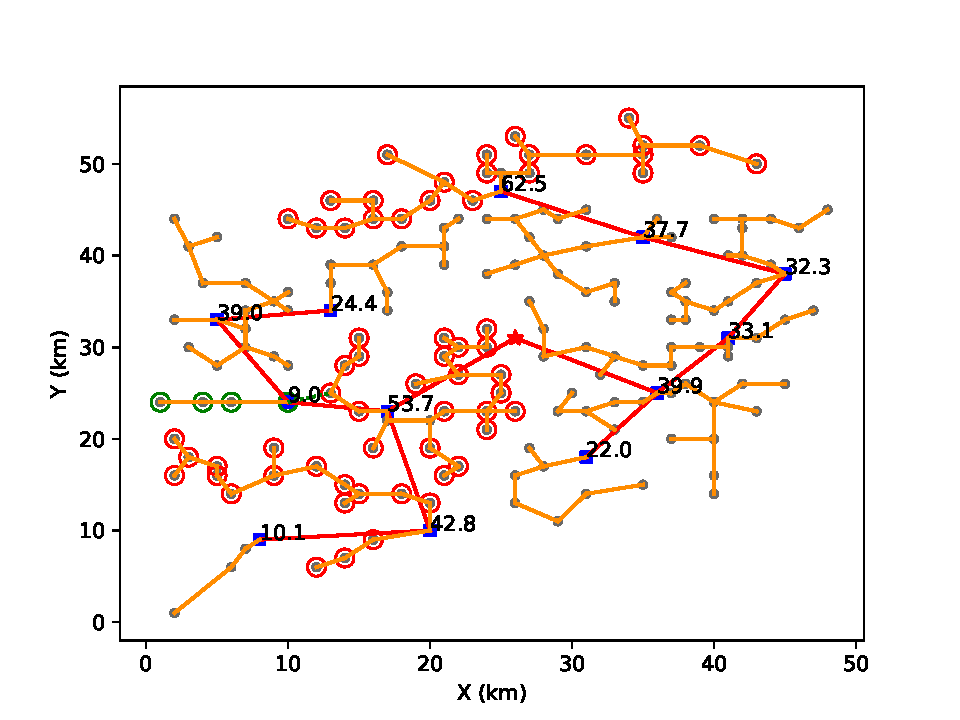
\includegraphics[width=0.99\textwidth]{figure/pipline_graft_connection_2.pdf}
        \subcaption{第3次嫁接的候选水站和$<u, v>$}
        \label{fig:pipline_graft_connection_2}
    \end{minipage}
    \begin{minipage}[c]{0.45\textwidth}
        \centering
        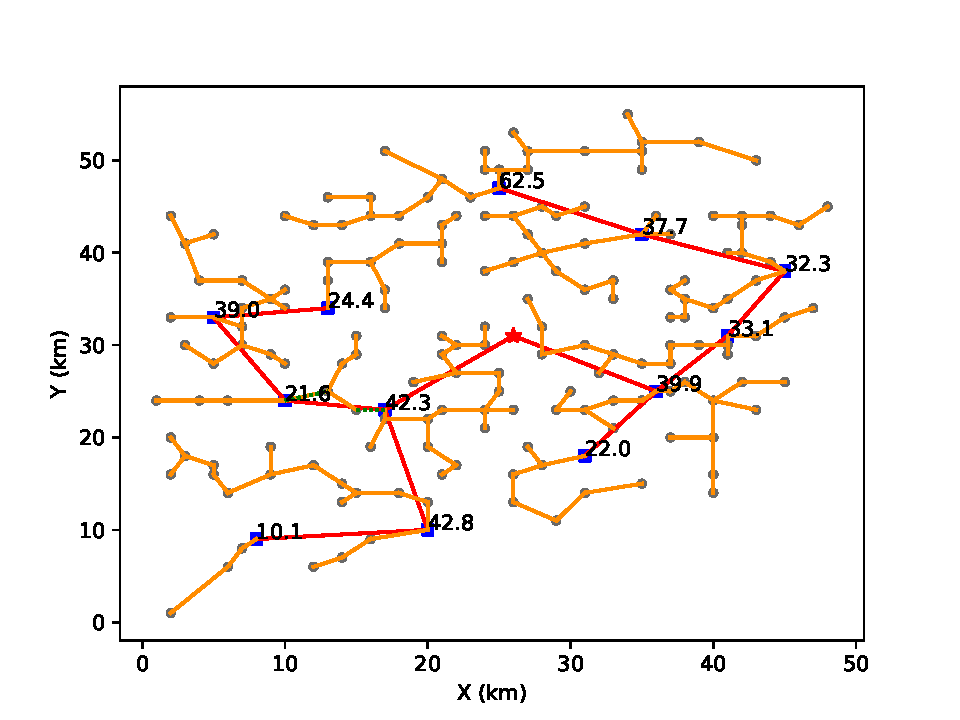
\includegraphics[width=0.99\textwidth]{figure/pipline_graft_cut_2.pdf}
        \subcaption{第3次嫁接断开的边}
        \label{fig:pipline_graft_cut_2}
    \end{minipage}
  \end{figure}
  
  \begin{figure}[!h]
    \centering
    \begin{minipage}[c]{0.45\textwidth}
        \centering
        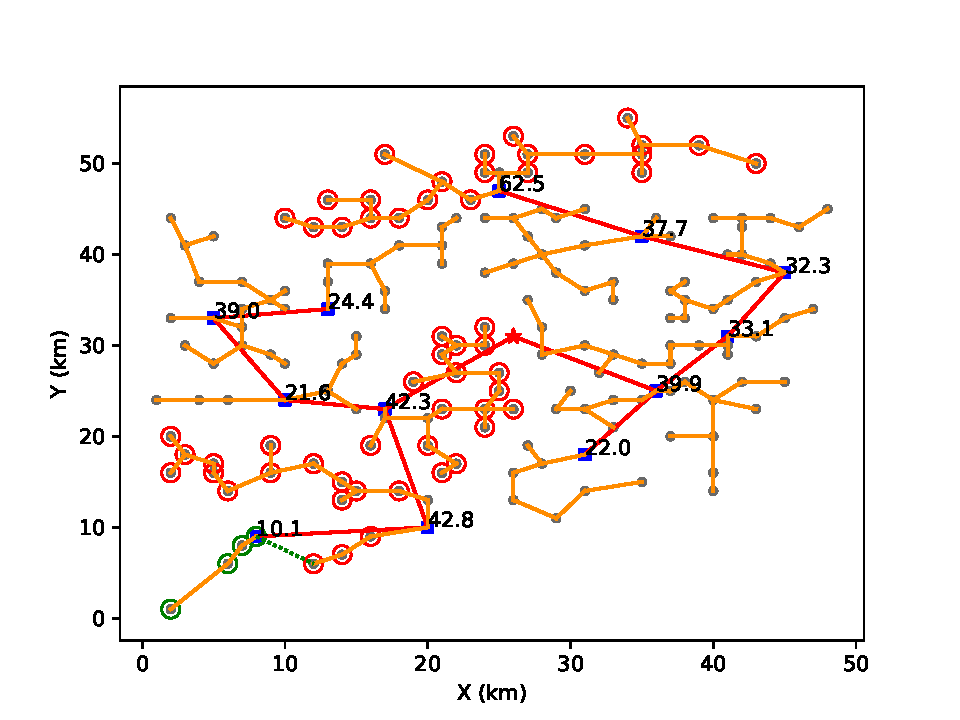
\includegraphics[width=0.99\textwidth]{figure/pipline_graft_connection_3.pdf}
        \subcaption{第4次嫁接的候选水站和$<u, v>$}
        \label{fig:pipline_graft_connection_3}
    \end{minipage}
    \begin{minipage}[c]{0.45\textwidth}
        \centering
        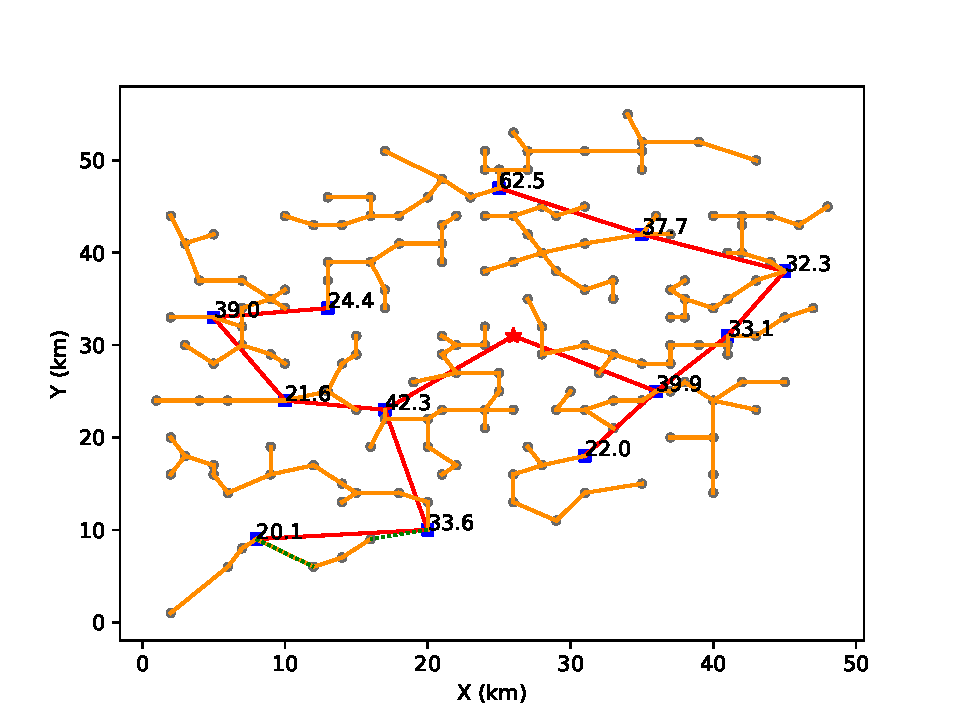
\includegraphics[width=0.99\textwidth]{figure/pipline_graft_cut_3.pdf}
        \subcaption{第4次嫁接断开的边}
        \label{fig:pipline_graft_cut_3}
    \end{minipage}
  \end{figure}
  
  \begin{figure}[!h]
    \centering
    \begin{minipage}[c]{0.45\textwidth}
        \centering
        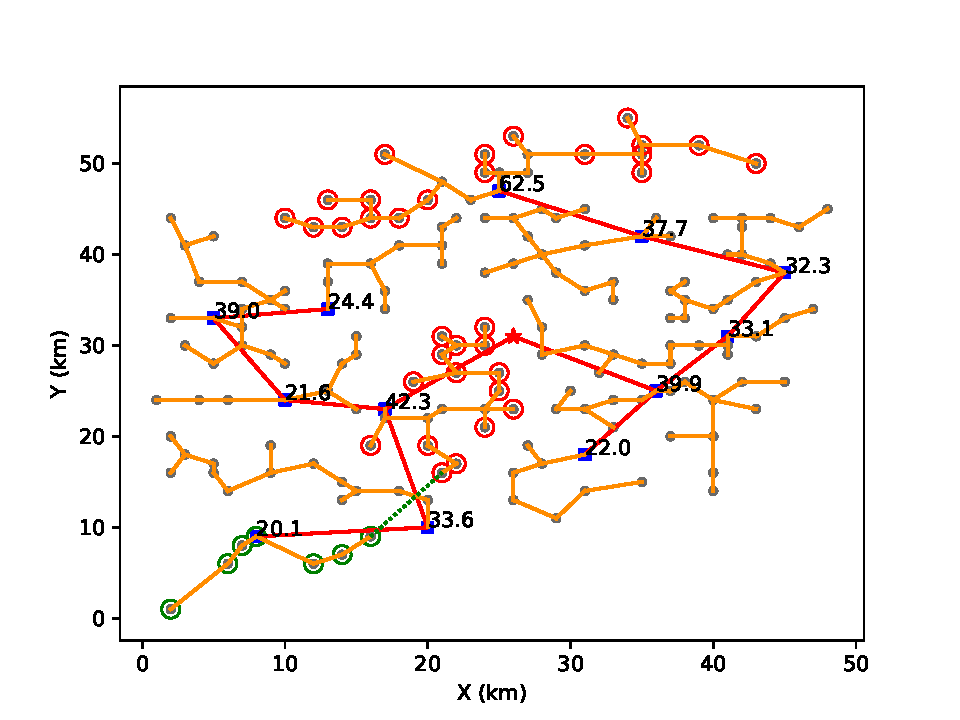
\includegraphics[width=0.99\textwidth]{figure/pipline_graft_connection_4.pdf}
        \subcaption{第5次嫁接的候选水站和$<u, v>$}
        \label{fig:pipline_graft_connection_4}
    \end{minipage}
    \begin{minipage}[c]{0.45\textwidth}
        \centering
        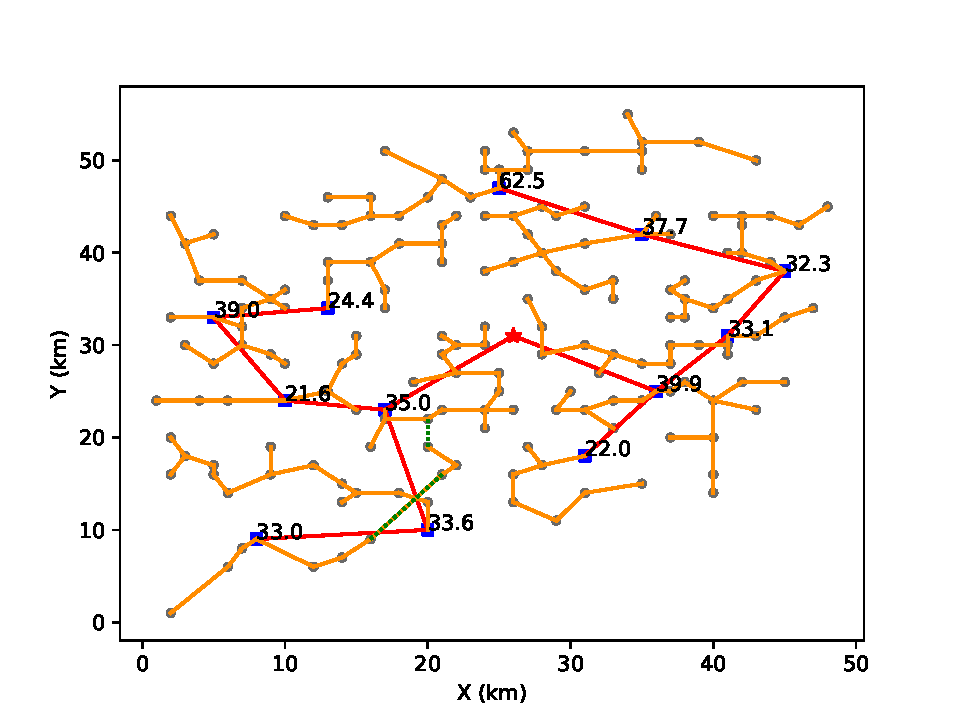
\includegraphics[width=0.99\textwidth]{figure/pipline_graft_cut_4.pdf}
        \subcaption{第5次嫁接断开的边}
        \label{fig:pipline_graft_cut_4}
    \end{minipage}
  \end{figure}
  
  \begin{figure}[!h]
    \centering
    \begin{minipage}[c]{0.45\textwidth}
        \centering
        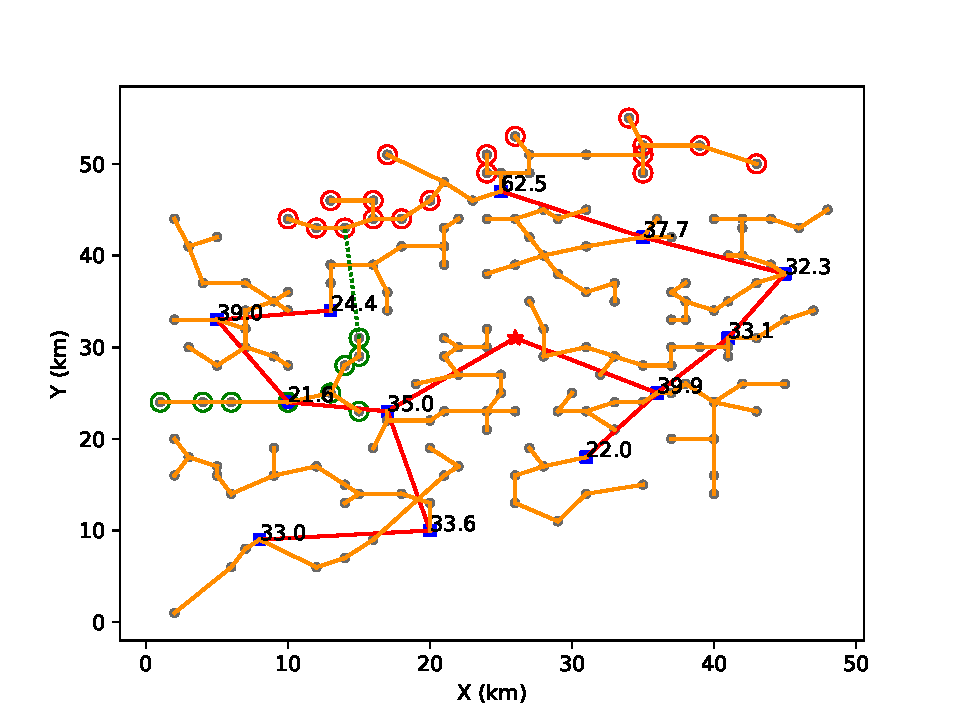
\includegraphics[width=0.99\textwidth]{figure/pipline_graft_connection_5.pdf}
        \subcaption{第6次嫁接的候选水站和$<u, v>$}
        \label{fig:pipline_graft_connection_5}
    \end{minipage}
    \begin{minipage}[c]{0.45\textwidth}
        \centering
        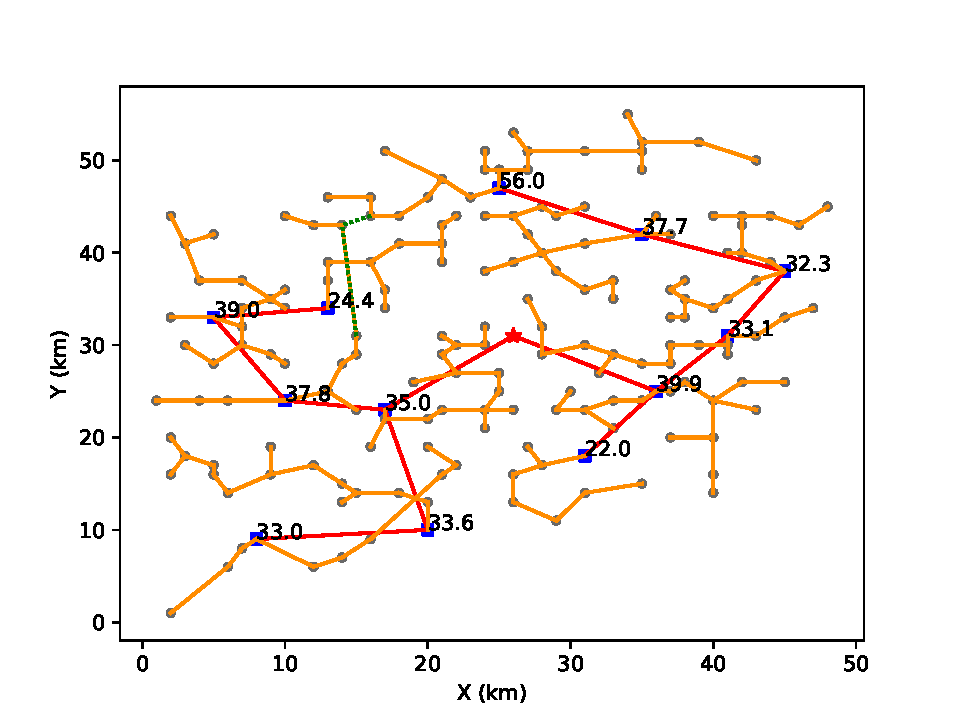
\includegraphics[width=0.99\textwidth]{figure/pipline_graft_cut_5.pdf}
        \subcaption{第6次嫁接断开的边}
        \label{fig:pipline_graft_cut_5}
    \end{minipage}
  \end{figure}
  
  \begin{figure}[!h]
    \centering
    \begin{minipage}[c]{0.45\textwidth}
        \centering
        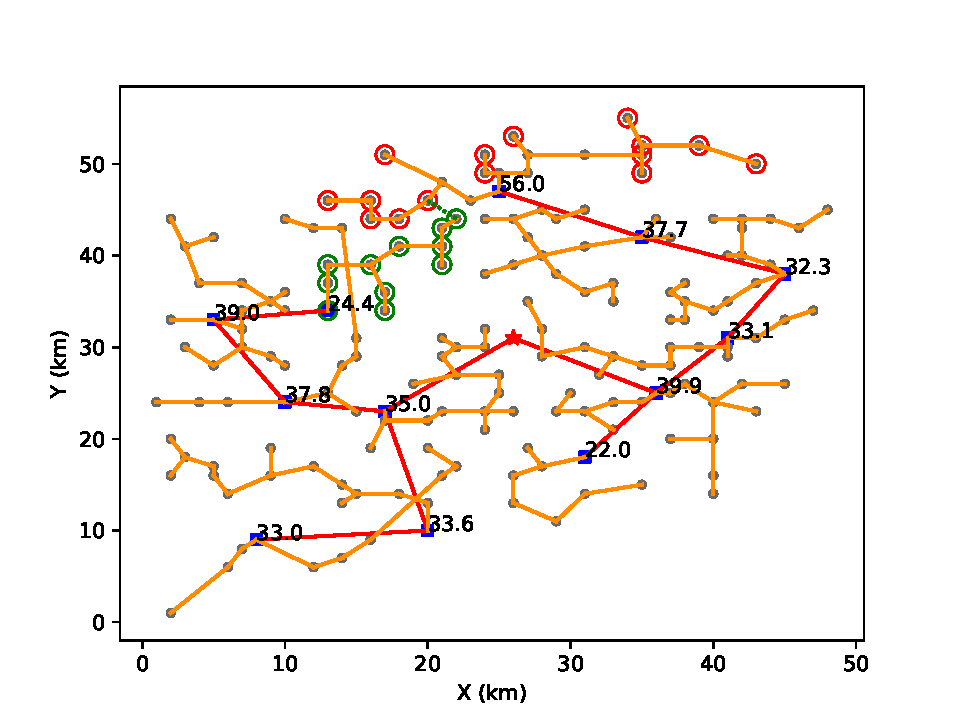
\includegraphics[width=0.99\textwidth]{figure/pipline_graft_connection_6.pdf}
        \subcaption{第7次嫁接的候选水站和$<u, v>$}
        \label{fig:pipline_graft_connection_6}
    \end{minipage}
    \begin{minipage}[c]{0.45\textwidth}
        \centering
        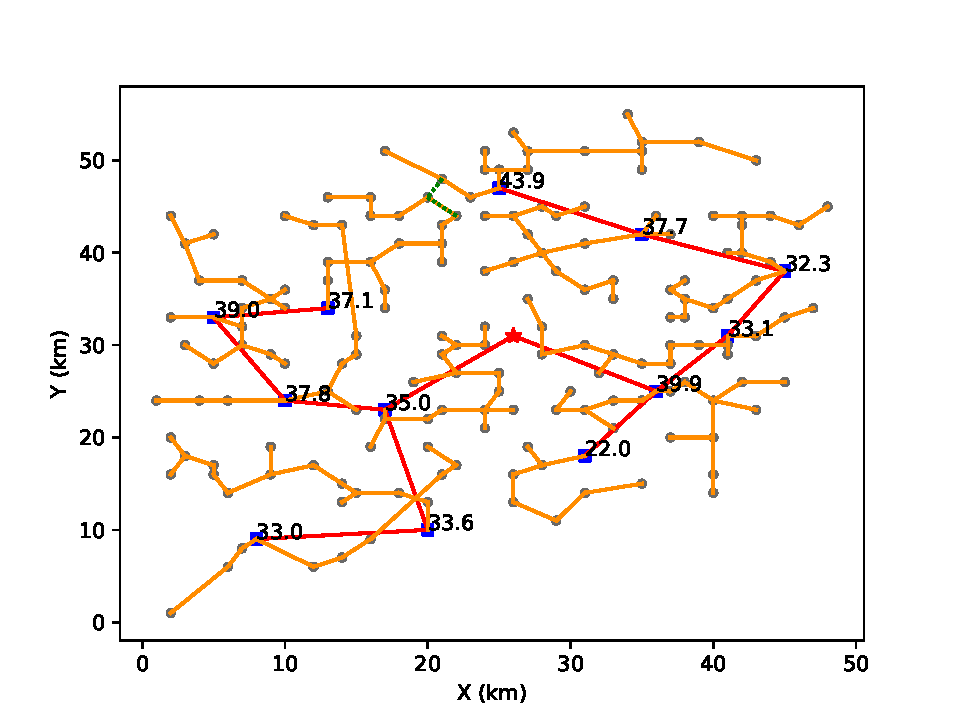
\includegraphics[width=0.99\textwidth]{figure/pipline_graft_cut_6.pdf}
        \subcaption{第7次嫁接断开的边}
        \label{fig:pipline_graft_cut_6}
    \end{minipage}
  \end{figure}
  
  \begin{figure}[!h]
    \centering
    \begin{minipage}[c]{0.45\textwidth}
        \centering
        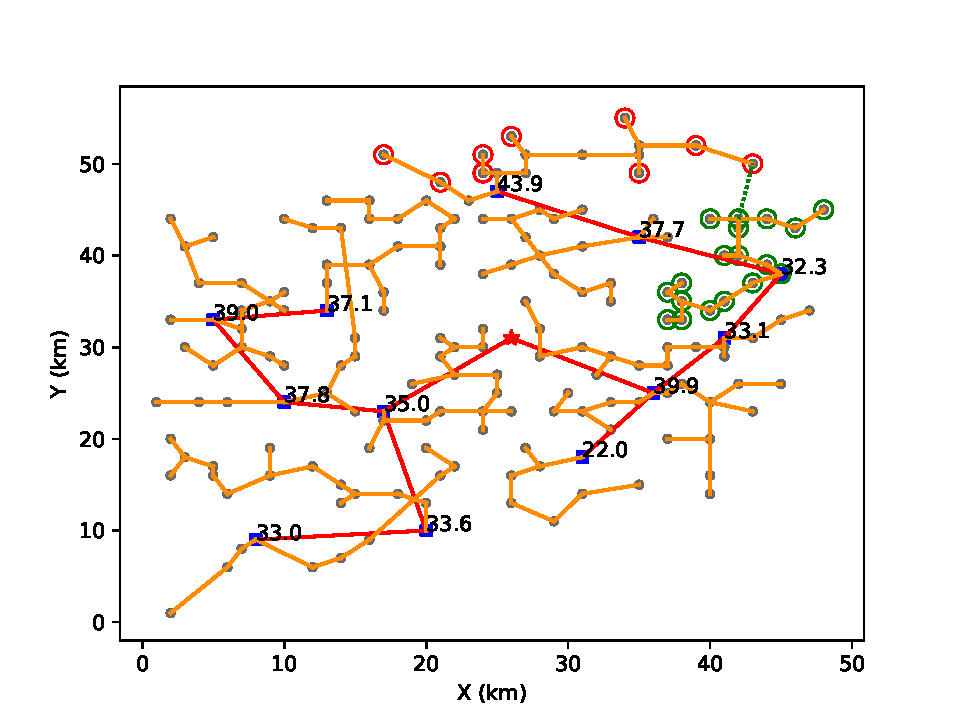
\includegraphics[width=0.99\textwidth]{figure/pipline_graft_connection_7.pdf}
        \subcaption{第8次嫁接的候选水站和$<u, v>$}
        \label{fig:pipline_graft_connection_7}
    \end{minipage}
    \begin{minipage}[c]{0.45\textwidth}
        \centering
        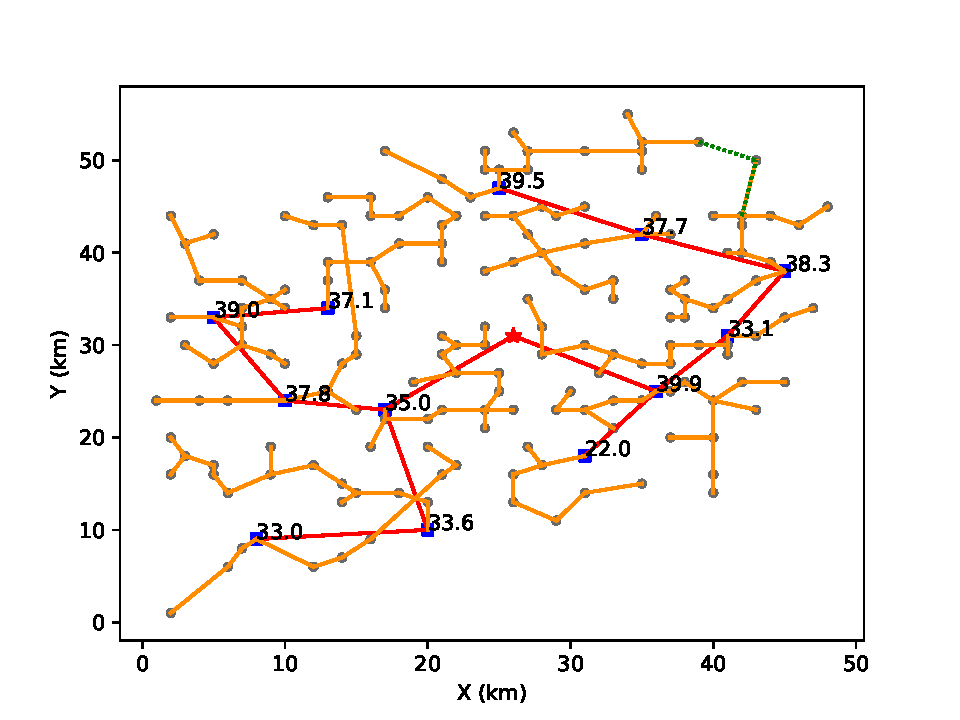
\includegraphics[width=0.99\textwidth]{figure/pipline_graft_cut_7.pdf}
        \subcaption{第8次嫁接断开的边}
        \label{fig:pipline_graft_cut_7}
    \end{minipage}
  \end{figure}
最终
嫁接后II级水管总长:425.94km。如\cref{fig:pipline_graft_cut_9}
\begin{figure}[!h]
  \centering
  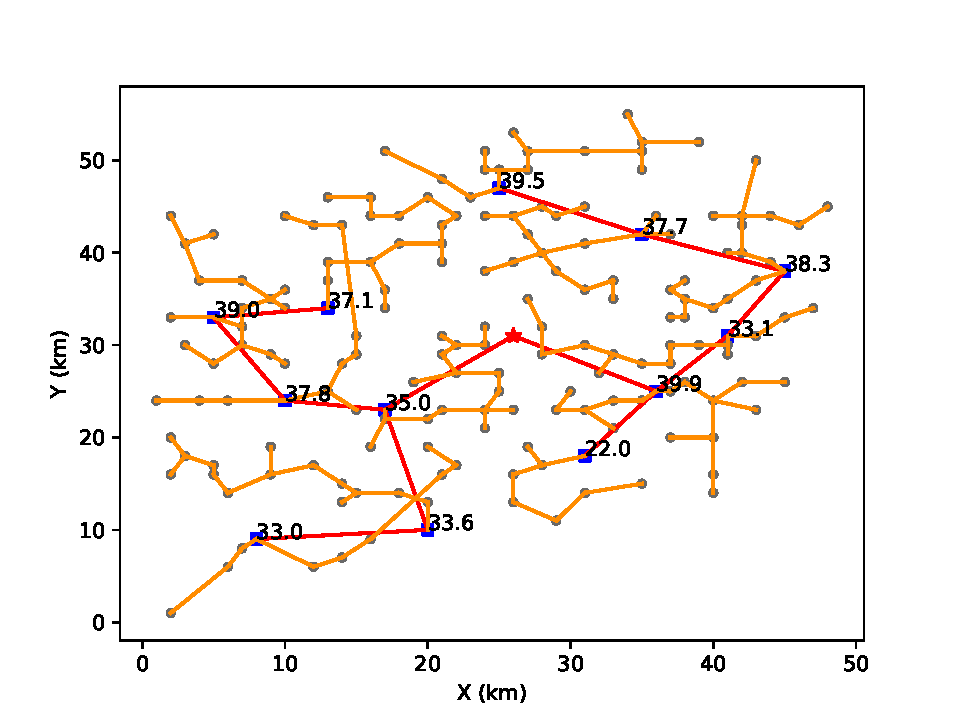
\includegraphics[width=.9\textwidth]{figure/pipline_graft_cut_9.pdf}
  \caption{问题3结果}
  \label{fig:pipline_graft_cut_9}
\end{figure}

\newpage

\section{模型总结与评估}
\subsection{优点}
\begin{itemize}
\item 在构建最优管道系统时,Prim算法可以寻找在当前情况下的最优解,并将新的站点纳入系统,在应对稠密多个连接点系统时具有优势。
\item 嫁接法兼顾了管线长度最小和一级水站的负载均衡,充分利用水站的空余负载,达到尽量减少升级水站数目的目的。
\end{itemize}
\subsection{缺点}
\begin{itemize}
\item Prim算法在进行边的选择时,会遍历所有边线,这样会导致算法具有较高时间复杂度。
\item

\end{itemize}
%参考文献
\section{参考文献}
  [1]冯立艳,何世伟,耿浩,关铁成.面向装配序列规划的最小生成树方法[J].机械设计与制造,2020(07):300-303.

  [2]李俊贤. 基于生成树算法的陆上风电场集电系统综合优化[D].电子科技大学,2020.
  
  [3]贺军忠,崔俊峰.基于Prim的局域网升级改造算法优化[J].廊坊师范学院学报(自然科学版),2020,20(01):24-26.
  
  [4]王佳敏,吴海燕.基于Prim算法的农村公路布局重要度最大树的求解与应用[J].公路,2019,64(06):162-166.
  

\newpage
%附录
\begin{appendices}
  \section{Python源代码}
  \begin{lstlisting}[language=python]
import numpy as np
import data
import plot
import functools
import time
from tqdm import tqdm
import collections

INF = np.inf
MAX_LOAD = 40
TRY_MAX_AVAILABLE_I = 5
TRY_MAX_PERCENTAGE = 0.9
DATA = data.Data()


# 计时装饰器
def timer(func):
    @functools.wraps(func)
    def wrapper(*args, **kwargs):
        begin_time = time.perf_counter()
        value = func(*args, **kwargs)
        end_time = time.perf_counter()
        run_time = end_time - begin_time
        print('{} 共用时:{} s'.format(func.__name__, run_time))
        return value
    return wrapper


class Tree:
    def __init__(self, edges):
        self.edges = set(edges)
        self.tree, self.front_station_of = self.edges_to_tree(edges)
        self.cal_length_from_all_station()
        self.IFirstID = DATA.stationNum[0]
        self.ILastID = DATA.stationNum[0] + DATA.stationNum[1]

    @staticmethod
    def distece_between(v, u):
        return DATA.distanceMat12[v, u]
    @staticmethod
    def edges_to_tree(edges):
        station = DATA.station012
        tree = dict()
        front_station_of = dict()
        for stationID in station.loc[station["classID"] != 0]["id"]:
            tree[stationID] = set()

        for k, v in edges:
            if k in tree:
                tree[k].add(v)
                front_station_of[v] = k
        return tree, front_station_of

    def cal_length_from_all_station(self):
        self.length_from_station = dict()
        station = DATA.station012
        IStationIDLst = station.loc[station["classID"] == 1]["id"]
        for IStationID in IStationIDLst:
            self.cal_length_from_station(IStationID)

    def cal_length_from_station(self, stationID):
        """
        递归求解从当前stationID输出的所有供水站管线长度和
        :param stationID:
        :return:
        """
        if len(self.tree[stationID]) == 0:
            self.length_from_station[stationID] = 0
            return 0
        elif stationID in self.length_from_station:
            return self.length_from_station[stationID]
        else:
            length = 0
            for next in self.tree[stationID]:
                length += DATA.distanceMat12[stationID, next]
                length += self.cal_length_from_station(next)
            self.length_from_station[stationID] = length
            return length

    def get_availableIStation_overloadIStationSet(self):
        availableIStation2availableLoad = dict()
        overloadIStationSet = set()
        for i in range(self.IFirstID, self.ILastID):
            load = self.length_from_station[i]
            if load < TRY_MAX_PERCENTAGE*MAX_LOAD:
                availableIStation2availableLoad[i] = MAX_LOAD - load
            elif load > MAX_LOAD:
                overloadIStationSet.add(i)
        return availableIStation2availableLoad, overloadIStationSet

    def get_grafting_candidate(self):
        availableI2Load, overloadIStationSet = self.get_availableIStation_overloadIStationSet()
        if len(availableI2Load) == 0:
            return None, None
        # 对availableLoad进行降序排列
        self.orderedAvailableI2Load = collections.OrderedDict(
            sorted(availableI2Load.items(), key=lambda t: -t[1])
        )

        self.orderedAvailableI2Station = collections.OrderedDict()
        for i, availableI in enumerate(self.orderedAvailableI2Load.keys()):
            self.orderedAvailableI2Station[availableI] = set((availableI,))
            self.add_all_next_selectedAvailable(availableI, availableI)
            if i >= TRY_MAX_AVAILABLE_I:
                break

        self.orderedAvailableI2candidateOverload = collections.OrderedDict()
        for i, availableI in enumerate(self.orderedAvailableI2Load.keys()):
            self.orderedAvailableI2candidateOverload[availableI] = set()
            for overloadIstation in overloadIStationSet:
                self.add_all_next_candidateOverload(availableI, overloadIstation)
            if i >= TRY_MAX_AVAILABLE_I:
                break
        return self.orderedAvailableI2Station, self.orderedAvailableI2candidateOverload

    def add_all_next_selectedAvailable(self, availableI, stationID):
        """
        递归地把树中所有stationID的子节点加入self.orderedAvailableI2Station[]
        :param stationID:
        :return:
        """
        if len(self.tree[stationID]) == 0:
            # 无下一节点
            return
        for next in self.tree[stationID]:
            self.orderedAvailableI2Station[availableI].add(next)
            self.add_all_next_selectedAvailable(availableI, next)

    def add_all_next_candidateOverload(self, availableI, stationID):
        if len(self.tree[stationID]) == 0:
            # 无下一节点
            return
        for next in self.tree[stationID]:
            load = self.length_from_station[next]
            if load < self.orderedAvailableI2Load[availableI]:
                self.orderedAvailableI2candidateOverload[availableI].add(next)
            self.add_all_next_candidateOverload(availableI, next)

    def get_cutEdge(self, graftEdge, availableI):
        u, v = graftEdge
        graftEdgeLength = self.distece_between(u, v)
        if graftEdgeLength > self.orderedAvailableI2Load[availableI]:
            return None
        self.edges.add((u, v))
        stationID = v
        while self.length_from_station[self.front_station_of[stationID]] < \
                self.orderedAvailableI2Load[availableI]-graftEdgeLength:
            self.edges.discard((self.front_station_of[stationID], stationID))
            self.edges.add((stationID, self.front_station_of[stationID]))
            stationID = self.front_station_of[stationID]
        cutEdge = (self.front_station_of[stationID], stationID)
        self.edges.discard(cutEdge)
        self.tree, self.front_station_of = self.edges_to_tree(self.edges)
        self.cal_length_from_all_station()
        return cutEdge

class Prim:
    def __init__(self):
        self.pip1 = []
        self.pip1len = 0
        self.pip2 = []
        self.pip2len = 0

        self.solve1()
        self.solve2()
        self.solve3()
    @staticmethod
    def min_edge(selected, candidate, graph, idMap=None):
        """
        求已经确定的顶点集合与未选顶点集合中的最小边
        :param selected:
        :param candidate:
        :param graph:
        :param idMap: 将graph中的索引映射到station["ID"]
        :return:返回新增选择的编号以及记录的最小边的两个顶点的station["ID"]
        """
        v, u = 0, 0
        weights = np.zeros((len(selected), len(candidate)))
        selectedArr = np.array(list(selected))
        candidateArr = np.array(list(candidate))
        # 循环扫描已选顶点与未选顶点,寻找最小边
        for i in range(len(selected)):
            weights[i] = graph[selectedArr[i], candidateArr]
        minID = np.argmin(weights)
        i = selectedArr[minID // len(candidate)]
        j = candidateArr[minID % len(candidate)]

        if idMap is not None:
            v, u = idMap[i], idMap[j]
        else:
            v, u = i, j
        return j, v, u

    def prim(self, graph, selected=None, candidate=None, idMap=None):
        """"""
        if selected is None:
            selected = set((0,))
        if candidate is None:
            candidate = set(range(len(graph))) - selected
        # 顶点个数
        vertex_num = len(candidate)
        # 存储每次搜索到的最小生成树的边
        edges = []
        # 由于连接n个顶点需要n-1条边,故进行n-1次循环,以找到足够的边
        for i in range(vertex_num):
            # 调用函数寻找当前最小边
            selection, v, u = self.min_edge(selected, candidate, graph, idMap=idMap)
            # 添加到最小生成树边的集合中
            edges.append((v, u))
            # v是selected中的顶点,u为candidate中的顶点,故将u加入candidate,以代表已经选择该顶点
            selected.add(selection)
            # 同时将u从candidate中删除
            candidate.discard(selection)
        return edges

    def cal_length(self, edges):
        """
        求生成树的总长度
        :param edges:
        :return:生成树的总长度,平均长度
        """
        station = DATA.station012
        total_length = 0
        for edge in edges:
            x0, x1 = station["X"][edge[0]], station["X"][edge[1]]
            y0, y1 = station["Y"][edge[0]], station["Y"][edge[1]]
            total_length += np.sqrt((x0-x1)**2 + (y0-y1)**2)
        return total_length, total_length/len(edges)

    @timer
    def solve1(self):
        """
        使用prim算法求解第1问,I型II型管道的方案
        :return:
        """
        self.pip1 = self.prim(DATA.distanceMat01)
        print("I型管道{}条".format(len(self.pip1)))
        self.pip1len, self.pip1avglen = self.cal_length(self.pip1)
        print("total length: {}".format(self.pip1len))

        selectedNum = DATA.stationNum[0] + DATA.stationNum[1]
        print("selectedNum: {}".format(selectedNum))

        self.pip2 = self.prim(DATA.distanceMat12, selected=set(range(selectedNum)))
        print("II型管道{}条".format(len(self.pip2)))
        print(self.pip2)
        self.pip2len, self.pip2avglen = self.cal_length(self.pip2)
        print("total length: {}".format(self.pip2len))
        plot.plot_pipeline(DATA.station012, self.pip1, self.pip2)

        print("I型供水站总负载")
        self.tree2 = Tree(self.pip2)
        # print(self.tree2.length_from_station)
        station = DATA.station012
        IStationIDLst = station.loc[station["classID"] == 1]["id"]
        for IStationID in IStationIDLst:
            print("{}: {}, ".format(IStationID, self.tree2.length_from_station[IStationID]))

    @timer
    def solve2(self):
        """
        使用枚举和prim算法求解第2问,搜索升级两个二级水站后,II型管道总长度最小的方案
        :return:
        """
        vertex_num = len(DATA.distanceMat12)# 顶点个数
        selectedNum = DATA.stationNum[0] + DATA.stationNum[1]
        selected = set(range(selectedNum))
        candidate = set(range(vertex_num)) - selected
        candidateLst = list(candidate)
        self.min_lengthAfterUpgrade = self.pip2len

        trials = [(i, j) for i in range(1, len(candidateLst)) for j in range(i)]
        total_step = len(trials)
        for i, j in tqdm(trials):
            upgradeStationID = set((candidateLst[i], candidateLst[j]))
            selectedAfterUpgrade = selected | upgradeStationID
            pip2 = self.prim(DATA.distanceMat12, selected=selectedAfterUpgrade)
            pip2len, _ = self.cal_length(pip2)
            if pip2len < self.min_lengthAfterUpgrade:
                self.min_lengthAfterUpgrade = pip2len
                self.min_pip2 = pip2
                self.upgradeStationID = upgradeStationID

        print("分别升级{}".format(self.upgradeStationID))
        print("\n升级两个二级水站后的II型管道{}条".format(len(self.min_pip2)))
        print(self.min_pip2)
        print("II型管道最小总长度: {}".format(self.min_lengthAfterUpgrade))
        upgradeStation = DATA.station012.loc[self.upgradeStationID]
        station01AfterUpgrade = DATA.station01.append(upgradeStation).reset_index(drop=True)
        graphAfterUpgrade = DATA.get_distanceMat(station01AfterUpgrade)
        self.min_pip1 = self.prim(graphAfterUpgrade, idMap=station01AfterUpgrade["id"])
        print("\n升级两个二级水站后的I型管道{}条".format(len(self.min_pip1)))
        print(self.min_pip1)
        plot.plot_pipeline(DATA.station012, self.min_pip1, self.min_pip2,
                            upgradeStationID=list(self.upgradeStationID), name="pipelineAfterUpgrade")

    @timer
    def solve3(self):
        i = 0
        lastCutEdge = (-1, -1)
        while True:
            orderedAvailableI2Station, orderedAvailableI2candidateOverload =\
                self.tree2.get_grafting_candidate()
            if orderedAvailableI2Station is None:
                break
            for availableI in orderedAvailableI2Station.keys():
                cutEdge = None
                selectedAvailable = orderedAvailableI2Station[availableI]
                candidateOverload = orderedAvailableI2candidateOverload[availableI]
                if len(selectedAvailable) == 0 or len(candidateOverload) == 0:
                    continue
                # 调用函数寻找当前最小边
                selection, v, u = self.min_edge(selectedAvailable, candidateOverload,
                                                DATA.distanceMat12)
                plot.plot_tree(DATA.station012, self.pip1, self.tree2,
                                selectedAvailable, candidateOverload,
                                extraEdges=((v, u),),
                                name="pipline_graft_connection_{}".format(i))
                cutEdge = self.tree2.get_cutEdge((v, u), availableI)
                if cutEdge is not None:
                    break
            if cutEdge == lastCutEdge:
                break
            lastCutEdge = cutEdge
            plot.plot_tree(DATA.station012, self.pip1, self.tree2,
                            extraEdges=((v, u),), cutEdge=cutEdge, annotateIIStation=False,
                            name="pipline_graft_cut_{}".format(i))
            i += 1
        print("嫁接后II级水管总长:{}".format(self.cal_length(self.tree2.edges)[0]))


if __name__ == '__main__':
    p = Prim()
    
  \end{lstlisting}
  \begin{lstlisting}[language=python]
import matplotlib.pyplot as plt
import seaborn as sns
from matplotlib.backends.backend_pdf import PdfPages
import pandas as pd


def plot_mat(mat, save=True, name="mat"):
    plt.figure()
    plt.imshow(mat, cmap=plt.cm.hot)
    plt.colorbar()
    if save:
        pdf = PdfPages("img//{}.pdf".format(name))
        pdf.savefig()
        pdf.close()
    else:
        plt.show()
    plt.close()


def plot_map(station, save=True, pointSize=25, name="map"):
    # print(station["classID"])
    plt.figure()
    plt.scatter(station["X"], station["Y"], s=pointSize-10*station["classID"], c=station["classID"], cmap="Set1")
    plt.xlabel("X (km)")
    plt.ylabel("Y (km)")
    if save:
        pdf = PdfPages("img//{}.pdf".format(name))
        pdf.savefig()
        pdf.close()
    else:
        plt.show()
    plt.close()


def plot_pipeline(station, edges1, edges2, upgradeStationID=None, save=True, pointSize=50, name="pipeline"):
    plt.figure()
    for edge in edges2:
        x0, x1 = station["X"][edge[0]], station["X"][edge[1]]
        y0, y1 = station["Y"][edge[0]], station["Y"][edge[1]]
        plt.plot([x0, x1], [y0, y1], c="darkorange")
    for edge in edges1:
        x0, x1 = station["X"][edge[0]], station["X"][edge[1]]
        y0, y1 = station["Y"][edge[0]], station["Y"][edge[1]]
        plt.plot([x0, x1], [y0, y1], c="r")
    plt.scatter(station.loc[station["classID"] == 0]["X"],
                station.loc[station["classID"] == 0]["Y"],
                s=pointSize, marker="*", c="r")
    plt.scatter(station.loc[station["classID"] == 1]["X"],
                station.loc[station["classID"] == 1]["Y"],
                s=pointSize/2, marker="s", c="b")
    plt.scatter(station.loc[station["classID"] == 2]["X"],
                station.loc[station["classID"] == 2]["Y"],
                s=pointSize/4, c="dimgray")
    if upgradeStationID is not None:
        plt.scatter(station["X"][upgradeStationID],
                    station["Y"][upgradeStationID],
                    s=1.2*pointSize, marker="p", c="g")
    plt.xlabel("X (km)")
    plt.ylabel("Y (km)")
    if save:
        pdf = PdfPages("img//{}.pdf".format(name))
        pdf.savefig()
        pdf.close()
    else:
        plt.show()
    plt.close()


def plot_tree(station, edges1, tree, selectedAvailable=None, candidateOverload=None,
              upgradeStationID=None, extraEdges=None, cutEdge=None,
              annotateIIStation=True, save=True, pointSize=50, name="tree"):
    plt.figure()
    for edge in edges1:
        x0, x1 = station["X"][edge[0]], station["X"][edge[1]]
        y0, y1 = station["Y"][edge[0]], station["Y"][edge[1]]
        plt.plot([x0, x1], [y0, y1], c="r")
    for stationID, nextSet in tree.tree.items():
        for next in nextSet:
            if (stationID, next) == cutEdge:
                linestyle = (0, (1, 1))
                c = "g"
            else:
                linestyle = 'solid'
                c = "darkorange"
            x0, x1 = station["X"][stationID], station["X"][next]
            y0, y1 = station["Y"][stationID], station["Y"][next]
            plt.plot([x0, x1], [y0, y1], c=c, linestyle=linestyle)

    plt.scatter(station.loc[station["classID"] == 0]["X"],
                station.loc[station["classID"] == 0]["Y"],
                s=pointSize, marker="*", c="r")
    plt.scatter(station.loc[station["classID"] == 1]["X"],
                station.loc[station["classID"] == 1]["Y"],
                s=pointSize/2, marker="s", c="b")
    plt.scatter(station.loc[station["classID"] == 2]["X"],
                station.loc[station["classID"] == 2]["Y"],
                s=pointSize/4, c="dimgray")
    IStationIDLst = station.loc[station["classID"] == 1]["id"]
    for IStationID in IStationIDLst:
        plt.annotate('{:.1f}'.format(tree.length_from_station[IStationID]),
                      (station["X"][IStationID], station["Y"][IStationID]), fontsize=8
                      )
    if annotateIIStation:
        IIStationIDLst = station.loc[station["classID"] == 2]["id"]
        for IIStationID in IIStationIDLst:
            plt.annotate('{:.1f}'.format(tree.length_from_station[IIStationID]),
                          (station["X"][IIStationID], station["Y"][IIStationID]), fontsize=5
                          )
    if selectedAvailable is not None:
        for stationID in selectedAvailable:
            plt.scatter(station["X"][stationID],
                        station["Y"][stationID],
                        s=1.5*pointSize, c='', marker="o", edgecolors="g")
    if candidateOverload is not None:
        for stationID in candidateOverload:
            plt.scatter(station["X"][stationID],
                        station["Y"][stationID],
                        s=1.5*pointSize, c='', marker="o", edgecolors="r")
    if extraEdges is not None:
        for extraEdge in extraEdges:
            x0, x1 = station["X"][extraEdge[0]], station["X"][extraEdge[1]]
            y0, y1 = station["Y"][extraEdge[0]], station["Y"][extraEdge[1]]
            plt.plot([x0, x1], [y0, y1], c="g", linestyle=(0, (1, 1)))
    if upgradeStationID is not None:
        plt.scatter(station["X"][upgradeStationID],
                    station["Y"][upgradeStationID],
                    s=1.5*pointSize, marker="+", c="g")
    plt.xlabel("X (km)")
    plt.ylabel("Y (km)")
    if save:
        pdf = PdfPages("img//{}.pdf".format(name))
        pdf.savefig()
        pdf.close()
    else:
        plt.show()
    plt.close()
  \end{lstlisting}
  \begin{lstlisting}[language=python]
import pandas as pd
import numpy as np
import plot
import pickle

DATA_PATH = "data//data.xlsx"
DISTANCE01_MAT_PATH = "data//distanceMat01.txt"
DISTANCE12_MAT_PATH = "data//distanceMat12.txt"


class Data:
    def __init__(self):
        self.dataPath = DATA_PATH
        self.stationNum = [0, 0, 0]
        self.station012 = self.read_data()#[:120]
        self.station012[["id", "classID"]].astype(int)
        self.station01 = self.station012[self.station012["classID"] != 2].reset_index(drop=True)

        # try:
        #     self.distanceMat01 = np.loadtxt(DISTANCE01_MAT_PATH)
        # except IOError:
        self.distanceMat01 = self.get_distanceMat(self.station01)
        np.savetxt(DISTANCE01_MAT_PATH, self.distanceMat01)
        plot.plot_mat(self.distanceMat01, name="distanceMat01")

        # try:
        #     self.distanceMat12 = np.loadtxt(DISTANCE12_MAT_PATH)
        # except IOError:
        self.distanceMat12 = self.get_distanceMat(self.station012)
        self.distanceMat12[:, 0] = np.inf
        self.distanceMat12[0, :] = np.inf
        np.savetxt(DISTANCE12_MAT_PATH, self.distanceMat12)
        plot.plot_mat(self.distanceMat12, name="distanceMat12")

    def read_data(self):
        point = pd.read_excel(self.dataPath, sheet_name=0)
        point["classID"] = 0
        for i, c in enumerate(point["class"]):
            if c == "A":
                point.at[i, "classID"] = 0
                self.stationNum[0] += 1
                # 不要使用链式赋值: point["classID"][i]=0
                # ;SettingWithCopyWarning
            elif c.startswith("V"):
                point.at[i, "classID"] = 1
                self.stationNum[1] += 1
            elif c.startswith("P"):
                point.at[i, "classID"] = 2
                self.stationNum[2] += 1
        # print(point)
        plot.plot_map(point)
        return point

    def get_distanceMat(self, station):
        """
        计算供水站之间的距离矩阵
        :return:
        """
        distanceMat = np.zeros((len(station), len(station)))
        for i in range(distanceMat.shape[0]):
            for j in range(distanceMat.shape[1]):
                distanceMat[i, j] = np.sqrt(
                    (station["X"][i]-station["X"][j])**2 + (station["Y"][i]-station["Y"][j])**2
                )
        return distanceMat
  \end{lstlisting}
  \section{代码输出}
I型管道12条

total length: 120.94121490556834

selectedNum: 13

II型管道168条...

total length: 403.40460072346366

I型供水站总负载

1: 38.95757725714306, 

2: 10.053405777305734,

3: 9.0, 

4: 5.0, 

5: 53.68689099686257, 

6: 42.792623800487334, 

7: 112.40605624423273, 

8: 21.968621791713595, 

9: 4.23606797749979, 

10: 39.948122114152724, 

11: 33.09725435508211, 

12: 32.257980408983926, 

solve1 共用时:0.3172876 s

100%|██████████| 14028/14028 [10:53<00:00, 21.46it/s]

分别升级{89, 125}

升级两个二级水站后的II型管道166条... 

II型管道最小总长度: 392.0014764860308

升级两个二级水站后的I型管道14条...

solve2 共用时:654.0920646 s

嫁接后II级水管总长:425.94164799701247

solve3 共用时:7.801315299999942 s

进程已结束,退出代码 0

\end{appendices}

\end{document} 
